\subsection*{Mobile Robot Control with the ROS Navigation Stack}
Control of mobile robots through the ROS/USARSim interface is performed with the ROS navigation stack\footnote{http://www.ros.org/wiki/navigation}. The navigation stack is a 2D navigation stack that takes in information from odometry, sensor streams, and a goal pose and outputs safe velocity commands that are sent to a mobile base. The velocity commands are sent it the form of: x velocity, y velocity, theta velocity. Better performance of the navigation stack can be achieved by meeting the following requirements:
\begin{itemize}
\item[-] The robot has to use either differential drive or holonomic drive.
\item[-] A planar laser has the be mounted on the mobile base. This laser is used for map building and localization.
\item[-] The performance of the navigation stack will be best on robots that are nearly square or circular. It does work on robots of arbitrary shapes and sizes, but it may have difficulty with large rectangular robots in narrow spaces like doorways.
\end{itemize}

Although different models of mobile robot are developed in USARSim, the Pioneer 3-AT (P3AT) (Figure~\ref{fig:p3at}) appears to be a suitable candidate to use the navigation stack. The P3AT is a small square-shaped differential wheeled robot with a SICK Laser Measurement Sensor (LMS) 200 mounted on his base. The P3AT is also widely employed for research and prototyping applications involving mapping, navigation, monitoring, reconnaissance, vision, manipulation, cooperation, and other behaviors.

\begin{figure}[t!]
\centering
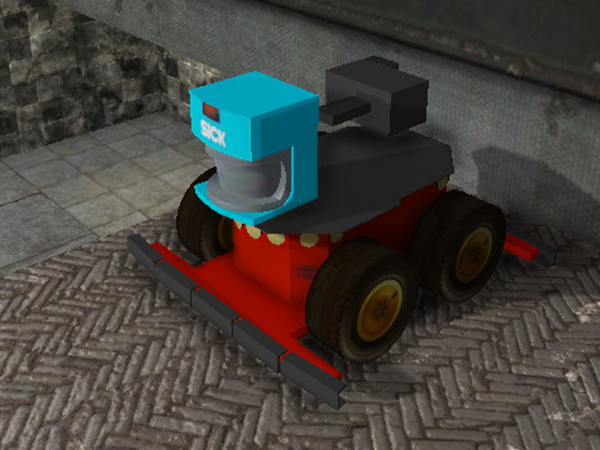
\includegraphics[width=4cm]{Figures/Robots/p3at.jpg}
\caption{Pioneer 3-AT (P3AT) in USARSim.}\label{fig:p3at}
\end{figure}




\subsubsection*{Low-level Navigation}
The ROS/USARSim interface allows the start-up and the control of the default P3AT base controllers by directly sending velocity commands to the base. This task was performed using the following commands:
\begin{enumerate}
\item\footnotesize{Bring up an environment in USARSim.        }
\item\footnotesize{\$roscore}
\item\footnotesize{\$roslaunch usarsim usarsim.launch}
\item\footnotesize{\$rosrun teleop\_twist\_keyboard teleop\_twist\_keyboard.py}
\item\footnotesize{\$rosrun gmapping slam\_gmapping scan:=lms200 \_odom\_frame:=odom}
\end{enumerate}

In step 1. an environment is started on server side (USARSim). If an environment is not up and running, passing messages between ROS and USARSim will fail. Step 2. starts \texttt{roscore}, a collection of nodes and programs that are a pre-requisites of a ROS-based system for ROS nodes to communicate. Step 3. launches the \texttt{usarsim.launch} file. This launch file contains information necessary to connect ROS to the computer running USARSim, to set up the appropriate robot (the P3AT in this case) at the correct location in the environment, to launch the proper ROS topics and to start the \texttt{RosSim} node. Step 4. starts the \texttt{teleop\_twist\_keyboard} node which sends velocity commands to the \texttt{RosSim} node through the computer keyboard. At this point, the P3AT can be controlled by keyboard teleop in the USARSim environment. Step 5. starts the node \texttt{slam\_gmapping} which transforms each incoming scan from the laser into the odometry tf frame to build a map. Here, the topic \texttt{scan} is used to create the map with the parameter \texttt{\_odom\_frame}, the frame attached to the odometry system.

\begin{figure}[t!]
\centering
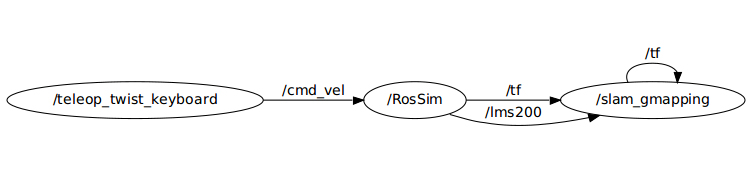
\includegraphics[width=9cm]{Figures/Misc/low-level.jpg}
\caption{Mobile robot control using \texttt{teleop}.}\label{fig:teleop}
\end{figure}

Figure~\ref{fig:teleop} is a graph generated by rxgraph with the option ``quiet". The graph illustrates the communication between the nodes \texttt{RosSim}, \texttt{teleop\_twist\_keyboard}, and \texttt{slam\_gmapping}. The keyboard inputs are converted in velocity commands and then communicated to the \texttt{RosSim} node on the topic \texttt{cmd\_vel}. \texttt{slam\_gmapping} uses the topics (\texttt{lms200}) and (\texttt{tf}) as inputs to build the map. To save the generated map, the following command is used:

\begin{itemize}
\item[]\$rosrun map\_server map\_saver
\end{itemize}

\begin{figure}[t!]
\centering
\subfigure[USARSim environment.]{\label{Fig:vmac-usarsim}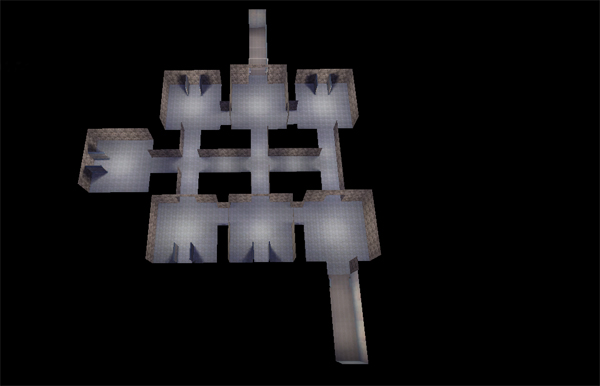
\includegraphics[width=4cm]{Figures/Misc/vmac-usarsim.jpg}}\qquad
\subfigure[Map of the environment.]{\label{Fig:vmac-usarsim-map}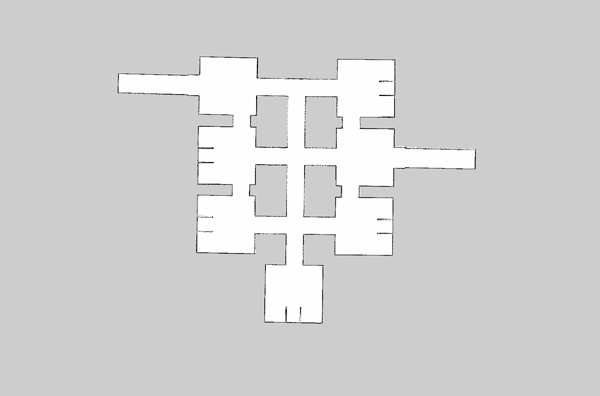
\includegraphics[width=4cm]{Figures/Misc/vmac-usarsim-map.jpg}}
\caption{Environment in USARSim and the corresponding map.}
\end{figure}
The generated map is stored in pair of files: a YAML file which describes the map meta-data and the image file that encodes the occupancy data. Figure~\ref{Fig:vmac-usarsim} is a bird view of the environment used to run the teleop command on the P3AT and Figure~\ref{Fig:vmac-usarsim-map} is the map generated by the \texttt{map\_saver} utility-command.



%\texttt{RosSim} publishes two topics for the odometry (\texttt{GndTruth} and \texttt{InsTest}), one topic to keep track of multiple coordinate frames over time \texttt{tf}, and a topic for the laser scanner (\texttt{lms200}).



\subsubsection*{High-level Navigation}
The ROS/USARSim interface also provides navigation at high level of the navigation stack. At this level, goals are sent to the P3AT to move to a particular location in the environment. Navigation at height level is possible with the action specification for \texttt{move\_base}. This package provides an implementation of an action (\texttt{actionlib}) that, given a goal in the world, will attempt to reach it with a mobile base. The \texttt{move\_base} node provides a ROS interface for configuring, running, and interacting with the navigation stack on a robot. The \texttt{move\_base} node links together a global and local planner to accomplish its global navigation task.

\begin{figure}[t!]
\centering
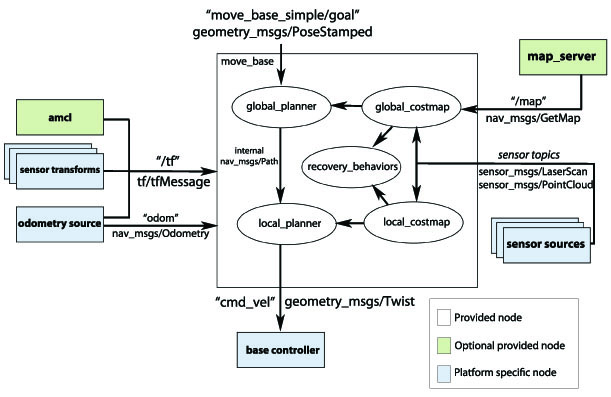
\includegraphics[width=10cm]{Figures/Misc/Navigation_Stack.jpg}
\caption{Navigation stack setup using \texttt{move\_base}.}\label{fig:navigation_stack}
\end{figure}

Figure~\ref{fig:navigation_stack} depicts a high-level view of the \texttt{move\_base} node and its interaction with other components of the navigation stack. The white components are required components, the green components are optional components, and the blue components must be created for each robot platform. The white and green components are already implemented. For the navigation stack to work properly for the P3AT, the nodes and topics generated should match the configuration of the \texttt{move\_base} node with the navigation stack.


Before running the \texttt{move\_base} node on the P3AT, localization, mapping and navigation information are filled in the \texttt{move\_base.launch} file:
\begin{itemize}
 \item [-] Localization uses map, laser data, and odometry to situate the robot in relation to the environment. The \texttt{amcl} and the \texttt{map\_server} nodes are necessary for robot localization. \texttt{amcl} is a probabilistic localization system for a robot moving in 2D and implements the KLD-sampling\cite{DIETER.IJRS.2003}. The \texttt{amcl} node is launched from the examples directory of the amcl package.
% and is included in \texttt{move\_base.launch} as one of its parameters.
\item [-] The \texttt{map\_server} node uses an {\it a priori} map generated by the \texttt{map\_saver} command-line utility. The example described in this paper uses the map depicted in Figure~\ref{Fig:vmac-usarsim-map} and its corresponding YAML file.
\item [-] The navigation stack uses cost-maps files (YAML files) to store information about obstacles in the world:
\begin{itemize}
\item [-] A global cost-map for creating long-term plans.
\item [-] A local cost-map for local planning and obstacle avoidance.
\item [-] A common cost-map file which stores configuration options used by the global and local cost-maps.
\end{itemize}
\item [-] The navigation stack uses a base local planner to compute velocity commands to send to the robot. Information on the base local planner is stored in a YAML file which sets configuration options based on the specs of the robot.
\end{itemize}

Once the \texttt{move\_base.launch} file is set up with the appropriate configuration options, the \texttt{move\_base} node is run with the following command:

\begin{itemize}
\item[]\$roslaunch move\_base.launch
\end{itemize}

To send commands to the P3AT, the package \texttt{simple\_navigation\_goals} was created (based on~\cite{SendingSimpleGoals}). The new package mainly includes the action specification for \texttt{move\_base}, an action client used to communicate with the action named \texttt{move\_base} that adheres to the MoveBaseAction interface, and a goal to send to \texttt{move\_base}. Sending commands through the code to the P3AT is performed by starting the executable for the \texttt{simple\_navigation\_goals} package:

\begin{itemize}
\item[]\$./bin/simple\_navigation\_goals
\end{itemize}

\begin{figure}[h!]
\centering
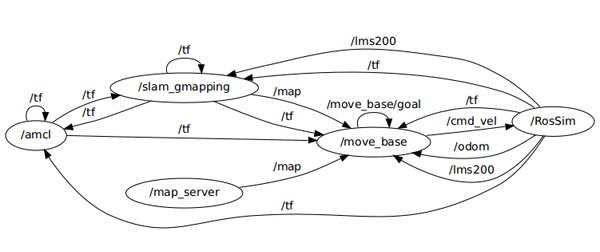
\includegraphics[width=10cm]{Figures/Misc/move_base.jpg}
\caption{Mobile robot control with move\_base.}\label{fig:movebase}
\end{figure}

Figure~\ref{fig:movebase} is a graph generated by rxgraph with the option ``quiet". The graph depicts the nodes and topics involved while sending a goal to move the P3AT at high level of the navigation stack. A parallel comparison of this graph with the navigation stack setup diagram (Figure~\ref{fig:navigation_stack}) reveals that the blue components have been implemented and the grey components were properly used. The node \texttt{move\_base} receives messages on the topic \texttt{tf} from the nodes \texttt{amcl}, \texttt{RosSim}, and \texttt{slam\_mapping}. \texttt{RosSim} publishes Odometry (\texttt{odom}) and sensor information (\texttt{lms200}) to \texttt{move\_base}. The optional node \texttt{map\_server} publishes the topic \texttt{map} to \texttt{move\_base}. Incoming messages are interpreted by \texttt{move\_base} which outputs velocity commands on the topic \texttt{cmd\_vel} to be sent to the node \texttt{RosSim}.
